The presented optimization problem employs binary decision variables and a single aggregated objective function with crisp parameter values to provide a clear, tractable, and straightforward formulation. Such a representation is very practical due to its computational efficiency, interpretability, and ease of implementation using standard optimization solvers. However, this framework neglects the uncertainty, imprecision, and conflicting nature of  real-world criteria, such as varied stakeholder preferences, uncertain resource availability, or imprecise risk estimations. Some of these aspects are precisely what we aim to model in this chapter to help a single decision maker select a specific schedule from a pool of feasible solutions. \\

The following section provides a detailed explanation of how the decision matrix (see table \ref{tab:dm_matrix}) is obtained by defining their attributes and explaining how different schedules (solutions) were computed using 3 of the top performing algorithms from the competition.

\subsection{Alternative Generation}

The analysis evaluates a pool of alternative schedules obtained from three leading algorithms submitted to the Roadef2020 challenge. These algorithms were selected from among the 13 finalists as they were the only ones that had their compiled solution code publicly available. These top performing solutions include the overall winning algorithm by Buljubašić and Vasquez\cite{top1} (Team S34) which secured first place, the matheuristic by Parreño et~al.\cite{ConsueloRoadef} (Team S56) which ranked third overall, and the algorithm by Marco Langiu\cite{top5} (Team J73) which won the junior category and ranked fifth overall.\\



The winning algorithm (S34) employs a scenario-penalisation matheuristic, which begins by solving a relaxed version of the problem with low penalties for constraint violations. It then iteratively increases these penalties, gradually guiding the search from initially cheap but infeasible solutions towards high-quality, feasible ones. The third-place solution (S56) follows a structured three-phase pipeline: it first generates multiple diverse schedules using a randomized greedy construction, refines them with a systematic local search, and finally uses an exact solver to optimally re-plan only the most critical activities. In contrast, the junior-winning algorithm (J73) relies almost entirely on a single mathematical model (Mixed-Integer Linear Programming), with its competitiveness stemming from a very effective greedy heuristic used to generate a high-quality initial solution to dramatically accelerate the exact solver.\\

Each algorithm was ran on the instance \texttt{X12} with different maximum computation times (180s, 300s, 500s, 700s, and 900s) and three different random seeds (42, 33, 73) on a GIGABYTE AORUS 15 BSF laptop with a 13th Gen Intel Core i7-13700H CPU and 16GB of DDR5-4800 RAM. This amounts to a total of 45 solutions (15 solutions per algorithm). However, the algorithm from Langiu failed to find feasible solutions in 4 of the setups, leaving a total of 41 solutions. The heat map (figure \ref{fig:dif_sol}) reveals that solutions 30-41 contain identical intervention schedules. Since these represent repeated solutions, only one representative (solution 30) will be kept, leaving us with 29 distinct solutions for analysis.

\begin{figure}[ht]
    \centering
    \includegraphics[width=0.8\textwidth]{ch3/figures/diff_sol.png}
    \caption{Heat map showing the count of different scheduled interventions between each pair of solutions. Solutions 30-41 are identical and correspond to the algorithm from Langiu.}
    \label{fig:dif_sol}
\end{figure}




\subsection{Retriving the physical location of the interventions}
One of the assumptions that will be made is that there is a component of the risk that comes from the location of an intervention. This is intuitive since interventions in densely populated areas or near critical infrastructure likely carry higher risks than those in remote locations. However, location is not the only factor, the risk also depends on other variables like the type of maintenance work. \\

Therefore, we will attempt to infer the approximate location of the interventions stating the following:
\begin{notation}{Assumption 1:}
    Two interventions \(i\) and \(j\) are close if their overall mean risks (averaged accross all possible start times and scenarios)
    \[
    \overline{r}_t^{(i)} = \frac{1}{\left|\mathcal{T}_i\right|}\sum_{\mathcal{T}_i}\mu_t^{(i,\tau)}, 
    \qquad \text{where }\mu_t^{(i,\tau)} \coleq \frac{1}{|S|}\sum_{s\in S} \mathrm{risk}_{s,t}^{(i,\tau)}, \quad
    \mathcal{T}_i\coleq \{\tau\in \N:\,1\leq \tau \leq T-d_{i,\tau}\}
    \]
    vary in the same direction, i.e.,
    \[
    \operatorname{sgn}\Big(\overline{r}_{t+1}^{(i)}-\overline{r}_t^{(i)}\Big)=\operatorname{sgn}\Big(\overline{r}_{t+1}^{(j)}-\overline{r}_t^{(j)}\Big),\quad t\in\{1,\dots , T-1\}
    \]
    This affirms that the risk variation of an intervention over time is strongly correlated with its location.
    \end{notation}


In practice, this condition will rarely hold for all time periods $t$. However, we can use it to define a similarity measure between interventions by counting how often their risk variations align. Specifically, for each pair of interventions $(i,j)$, we compute a similarity score by adding 1 when their risk variations match in sign and subtracting 1 when they differ. Then it is normalized to the interval $[-1,1]$. This yields a symmetric similarity matrix that captures the degree of correlation between intervention risks over time.

\begin{remark}
    By definition, an intervention has a correlation of 1 with itself.
\end{remark}

Notice that not all correlation values provide information about the closeness between interventions. Only positively correlated interventions can be considered "close" to some extent. However, we cannot determine how far apart negatively correlated interventions should be. Therefore, these negative correlations will be set to \texttt{NaN} and treated as missing values.\\

There is not enough information to assign a specific distance value between 2 close points, but following assumption 1: the higher the correlation between two interventions, the stronger the indication that they are close to each other. Therefore, the algorithm proposed to recover a map from a distance matrix is: non-metric weighted Multi-Dimensional Scaling (MDS):

\begin{itemize}
    \item \textbf{MDS:} Given a distance matrix (or dissimilarity matrix), it minimizes a stress function (\ref{eq:stress}) to find an embedding in a specified number of dimensions (in our case, 2 dimensions).
    \item \textbf{Non-metric:} Instead of using the magnitude of the distances, it only considers the ordinal information induced by those values. Higher correlations indicate closer distances, but the size of the difference between correlations is not necessarily proportional to the actual distances between interventions.
    \item \textbf{Weighted:} Each distance's contribution to the stress function is weighted by its correlation value, reflecting higher confidence in our assumption when correlations are stronger.
\end{itemize}

\begin{remark}
    The dissimilarity/distance matrix is obtained through a linear transformation of the previously defined similarity matrix:
    \begin{align*}
        \text{NaN} &\rightarrow \text{NaN} \\
        \text{cor}_{ij} &\rightarrow \text{dist}_{ij} = 1-\text{cor}_{ij}, \quad \text{where } \text{cor}_{ij} \in [0,1]
    \end{align*}
\end{remark}


\subsubsection*{Non-metric Weighted MDS with SMACOF \cite{smacof}:}
\paragraph{Problem Formulation .} Let us assume we have $n$ objects, and an $n\times n$ matrix of observed dissimilarities 
\[
\Delta = \bigl[\delta_{ij}\bigr],
\]
where $\delta_{ij} \ge 0$ and each pair of objects $(i,j)$ is assigned a weight $w_{ij}\ge 0$. The goal of \emph{non-metric} weighted MDS is to find an embedding of these objects as points $\mathbf{x}_1,\dots,\mathbf{x}_n$ in $\mathbb{R}^p$ (collectively denoted by $X \in \mathbb{R}^{n\times p}$), such that the pairwise distances $d_{ij}(X) = \|\mathbf{x}_i - \mathbf{x}_j\|$ (usually Euclidean) respect the \emph{rank ordering} of $\delta_{ij}$.

Formally, non-metric MDS replaces $\delta_{ij}$ with a \emph{monotonic transformation} $f(\cdot)$, yielding
\[
\hat{\delta}_{ij} = f(\delta_{ij}),
\]
subject to the isotonic constraint:
\[
\delta_{ij} < \delta_{kl} 
\quad \Longrightarrow \quad 
f(\delta_{ij}) \;\le\; f(\delta_{kl}).
\]
In case of a tie $(\delta_{ij} = \delta_{kl} )$, disparities are allowed as long as they maintain the correct ordering with respect to non-tied values.

We then define the \emph{weighted STRESS} function:
\begin{equation}
\mathrm{STRESS}(X,\hat{\Delta}) 
\;=\;
\frac{\sum_{i<j} w_{ij}\,\bigl(\hat{\delta}_{ij} \;-\; d_{ij}(X)\bigr)^2}{\sum_{i<j} w_{ij}\,d_{ij}(X)^2},
\label{eq:stress}
\end{equation}
where $\hat{\Delta}$ denotes the matrix $\bigl[\hat{\delta}_{ij}\bigr]$.  
The goal is to minimize this STRESS with respect to both $X$ and the (monotonic) mapping $f$. Missing values are simply not taken into account in the sum (which is equivalent to setting their weight to 0).

\paragraph{Solution via SMACOF}\label{sec:smacof-solution}
\emph{Scaling by MAjorizing a COmplicated Function} is an iterative algorithm that provides a stable, monotone-convergent framework for MDS. Unlike Kruskal's classic method, which uses gradient-based updates to move the configuration $X$, SMACOF replaces the gradient step with a \emph{majorization step} that guarantees non-increasing STRESS accross iterations. This is typically more numerically stable and better at handling large amounts of missing data.

The algorithm alternates between two main steps:

\begin{enumerate}
  \item \textbf{Initialization}
    \begin{enumerate}[(a)]
      \item Collect all non-missing dissimilarities $\{\delta_{ij}\}$ and set the corresponding weights $w_{ij}$ (with $w_{ij}=0$ for missing values).
      \item Choose an initial configuration $X^{(0)} \in \mathbb{R}^{n \times p}$ (e.g., via random placement or classical MDS).
    \end{enumerate}

  \item \textbf{Iterative Steps}
    \begin{enumerate}[(a)]
      \item \textbf{Optimal Scaling (Isotonic Regression):} \\
      Given the current configuration $X^{(t)}$, compute the Euclidean distances
      \[
        d_{ij}\bigl(X^{(t)}\bigr)=\|x_i^{(t)} - x_j^{(t)}\|,
      \]
      and determine the disparities by solving
      \[
        \min_{f\,:\, \text{non-decreasing}} \sum_{i<j} w_{ij}\,\Bigl(f(\delta_{ij}) - d_{ij}\bigl(X^{(t)}\bigr)\Bigr)^2.
      \]
      In practice, weighted isotonic regression (e.g., via the Up-and-Down-Blocks Algorithm\footnote{Up-and-Down-Blocks is a specific implementation strategy for PAVA (Pool-Adjacent-Violators Algorithm) that can be optimized for efficiency and linear time complexity. There are other possible implementations of PAVA that could be used.\cite{PAVA}}, see algorithm \ref{algo:Up-and-Down-Blocks}) is applied to obtain $\hat{\delta}_{ij}=f(\delta_{ij})$, ensuring that the transformed dissimilarities preserve the original rank order.
      
      \item \textbf{Majorization Update (Guttman Transform):} \\
      With the disparities $\hat{\Delta}=\{\hat{\delta}_{ij}\}$ fixed, 
      SMACOF constructs a quadratic majorizing function $Q\bigl(X, X^{(t)}\bigr)$ satisfying
      \[
        \mathrm{STRESS}(X,\hat{\Delta}) \le Q\bigl(X, X^{(t)}\bigr), \quad \text{with equality when } X = X^{(t)}.
      \]
      Minimizing $Q\bigl(X, X^{(t)}\bigr)$ leads to a closed-form update via the Guttman transform:
      \[
        X^{(t+1)} = V^{+}B\bigl(X^{(t)}\bigr)X^{(t)},
      \]
      \hspace{1em}where the constant matrix \(V\) is defined by
          \[
            V = \frac{1}{2}\sum_{i=1}^n \sum_{j=1}^n w_{ij}\,A_{ij}, \qquad \text{where }A_{ij} = (e_i - e_j)(e_i - e_j)^T,
          \]
          \hspace{1em}with \(e_i\) denoting the \(i\)th standard basis vector. Note that \(A_{ij} = A_{ji}\), and \(A_{ii} = 0\). The factor \(\frac{1}{2}\) accounts for double counting of symmetric terms. \(V\) is positive semidefinite and singular. Its Moore-Penrose inverse is denoted by \(V^{+}\).\\

        \hspace{1em}And the matrix \(B\bigl(X^{(t)}\bigr)\) is defined element-wise by
          \[
            B\bigl(X^{(t)}\bigr) = \frac{1}{2} \sum_i \sum_j w_{ij} \, \hat{\delta}_{ij} \, s_{ij}\bigl(X^{(t)}\bigr) \, A_{ij}, \quad \text{where } s_{ij}\bigl(X^{(t)}\bigr) = \begin{cases} \dfrac{1}{d_{ij}\bigl(X^{(t)}\bigr)} & \text{if } d_{ij}\bigl(X^{(t)}\bigr) \neq 0, \\ 0 & \text{otherwise} \end{cases}
          \]
          \hspace{1em}where \(d_{ij}\bigl(X^{(t)}\bigr)\) is the Euclidean distance between points \(i\) and \(j\) in the current configuration.

      By construction, the update satisfies
      \[
        \mathrm{STRESS}\bigl(X^{(t+1)},\hat{\Delta}\bigr) \le \mathrm{STRESS}\bigl(X^{(t)},\hat{\Delta}\bigr),
      \]
      ensuring a monotone decrease in stress.
    \end{enumerate}

  \item \textbf{Convergence Check}
    \begin{enumerate}[(a)]
      \item After updating $X^{(t+1)}$, recompute the stress. If the reduction in stress is below a predetermined tolerance (or no further improvement is observed), terminate the algorithm; otherwise, set $t\leftarrow t+1$ and return to the Optimal Scaling step.
    \end{enumerate}
\end{enumerate}


For details about the global linear convergence to a stationary point conditions of SMACOF see \cite{smacof}.

\begin{algorithm}[ht]
    \caption{Up-and-Down-Blocks Algorithm for Isotonic Regression \cite{modernMDS}}
    \label{algo:Up-and-Down-Blocks}
    \KwIn{A distance matrix $D=\{d_{ij}(X)\}$ from the current configuration $X$, and corresponding rank-ordered proximities $\{\delta_{ij}\}$ (with possible ties).}
    \KwOut{Disparities $\{\hat{d}_{ij}\}$ that are monotonic (non-decreasing) with respect to $\delta_{ij}$.}
    
    \tcp{Step 1: Initialization}
    \For{each pair $(i,j)$}{
        Set $\hat{d}_{ij} \gets d_{ij}(X)$\;
    }
    
    \tcp{Step 2: Iterative Pooling to Enforce Monotonicity}
    \While{there exists an index $k$ such that $\hat{d}_k > \hat{d}_{k+1}$}{
        \tcp{(a) Identify the first (leftmost) violation and initialize block $B$.}
        Let $k$ be the smallest index with $\hat{d}_k > \hat{d}_{k+1}$\;
        Set $B \gets \{k, k+1\}$\;
        Compute the block average:
        \[
        \bar{d} \gets \frac{\hat{d}_k + \hat{d}_{k+1}}{2}\,.
        \]
        and for each $i \in B$, set $\hat{d}_i \gets \bar{d}$\;
        
        \tcp{(b) Extend the block to the left.}
        \While{there exists an index $j = \min(B)-1$ such that $\hat{d}_j > \bar{d}$}{
            Update $B \gets B \cup \{j\}$\;
            Recompute 
            \[
            \bar{d} \gets \frac{1}{|B|}\sum_{i \in B} \hat{d}_i\,,
            \]
            and for each $i \in B$, set $\hat{d}_i \gets \bar{d}$\;
        }
        
        \tcp{(c) Extend the block to the right.}
        \While{there exists an index $l = \max(B)+1$ such that $\bar{d} > \hat{d}_l$}{
            Update $B \gets B \cup \{l\}$\;
            Recompute 
            \[
            \bar{d} \gets \frac{1}{|B|}\sum_{i \in B} \hat{d}_i\,,
            \]
            and for each $i \in B$, set $\hat{d}_i \gets \bar{d}$\;
        }
    }
    
    \tcp{Step 3: Handling Ties}
    For tied proximities (i.e., when $\delta_{ij} = \delta_{kl}$), the algorithm enforces overall monotonicity; that is, it does not explicitly force $\hat{d}_{ij} = \hat{d}_{kl}$. (If needed, a reordering step can ensure that disparities for tied proximities remain in non-decreasing order.)
    
    \tcp{Step 4: Normalization (for SMACOF/MDS)}
    Scale the final disparities so that
    \[
    \sum_{i<j} \hat{d}_{ij}^2 = \frac{n(n-1)}{2}\,.
    \]
    
    \Return $\{\hat{d}_{ij}\}$\;
\end{algorithm}

\begin{figure}[ht]
    \centering
    \includegraphics[width=\textwidth]{ch3/figures/points.png}
    \caption{Visualization of the resulting MDS map showing the relative positions of the interventions from \texttt{X12} in a two-dimensional space based on their dissimilarities derived from assumption 1.}
    \label{fig:mds_map}
\end{figure}




\subsection{Crisp Attributes}
\paragraph{Highest Concurrency:} In figure \ref{fig:concurrency} we can see the concurrency (i.e., the number of active interventions at a given time) of an example solution. The highest concurrency represents the maximum number of interventions being executed simultaneously at any time. In order to get the final score for the decision matrix, we normalize using the total number of interventions.

\begin{figure}[ht]
    \centering
    \includegraphics[width=\textwidth]{ch3/figures/Concurrency.png}
    \caption{Concurrent interventions over time for an example solution, showing the number of interventions being executed simultaneously at each time period. Colors are used to differentiate seasons.}
    \label{fig:concurrency}
\end{figure}



% \paragraph{Highest Risk:} This attribute measures the average worst-case risk across all interventions, where for each intervention we consider its maximum risk over all time periods and scenarios. Formally, we have:

% \[\operatorname{worst}^{(i,\tau)} \coleq \max_{t=1,\dots,d_{i,\tau}} \max_{s\in S} \mathrm{risk}_{s,t}^{(i,\tau)} \quad \text{where} \quad \text{highest\_risk} \coleq \frac{1}{|\mathcal{I}|}\sum_{i\in\mathcal{I}} \operatorname{worst}^{(i,\tau_i)}\]



\paragraph{Seasonality:} These are 3 attributes that indicate the proportion of total interventions active in each season (Winter, Summer, or Interseason). Note that the proportions sum to more than 1 since interventions can span multiple seasons.

\clearpage
\subsection{Fuzzy Attributes}
To enrich our decision-making model, we introduce four fuzzy attributes. These attributes evaluate the temporal distribution of interventions based on their size, risk, spatial proximity to each other, and environmental sensitivity. They are built upon the principles of fuzzy logic to translate crisp, quantitative data into a more expressive, linguistic framework suitable for multi-criteria analysis.\\

Our methodology for constructing these attributes follows a three-stage process. Crisp numerical data from each intervention is transformed into fuzzy sets over the intervention space, which represent the extent to which an intervention possesses a certain qualitative (linguistic) property. Second, for any given solution, 
we take the fuzzy subset of active interventions in each day and aggregate (add\footnote{Adding the memberships of a fuzzy set is equivalent to computing the cardinality of that fuzzy set.}) these memberships into a ''daily mass". This time series quantifies the total presence of that fuzzy property among the interventions active on each day of the planning horizon. Finally, we evaluate the temporal uniformity of this mass distribution using a scalar score derived from Shannon's entropy, allowing for a concise comparison between different solutions.\\

The initial stage, fuzzification, is achieved through one of two methods depending on the nature of the attribute. For properties based on distance, we define a \textbf{linguistic variable}. In this case, the linguistic variable \textit{Distance} defines 5 linguistic terms (close, mid-close, mid, mid-far, far), which are defined over a numerical base variable (distance in meters). The meaning of each linguistic term is captured by a membership function, $\mu(x)$, which assigns a compatibility degree in $[0, 1]$ to each value of the base variable. This degree of compatibility is conceptually distinct from probability, as it is not a frequency of any event. The membership functions the five terms are specified by trapezoidal and triangular numbers as shown in Figure~\ref{fig:fuzzy_distance}. Therefore, 5 values need to be chosen by the decision maker, which specify the boundaries of each fuzzy number.\\


\begin{figure}[!ht]
    \centering
    \includegraphics[width=\linewidth]{ch3/figures/Fuzzy distance.png}
    \caption{Fuzzy distance linguistic variable with close, mid-close, mid, mid-far and far membership functions. Five values (a,b,c,d,e) are required for defining the compatibility functions of the terms: 2 trapezoidal fuzzy numbers for close and far and 3 triangular fuzzy numbers for mid-close, mid and mid-far.}
    \label{fig:fuzzy_distance}
    \end{figure}

For attributes like intervention size and risk, where clear-cut boundaries are harder to set, we employ a data-driven approach using \textbf{fuzzy c-means clustering}. This unsupervised algorithm partitions the set of interventions into a specified number of clusters (in our case, five) based on their data. Unlike hard clustering, it assigns each intervention a membership degree to every cluster, reflecting partial associations. For example, an intervention could be 80\% medium and 20\% mid-large size. We apply this technique to the mean size and mean risk of each intervention, with the resulting cluster centroids, representing the prototypical value for each fuzzy category, shown in Table~\ref{tab:fuzzy_centroids}.

\begin{table}[!ht]
    \centering
    \begin{tabular}{lcc}
    \hline
    \textbf{Cluster Type} & \textbf{Size Centroids} & \textbf{Risk Centroids} \\
    \hline
    Small/Low & 389.36 & 972.16 \\
    Mid-small/Mid-low & 4,616.21 & 987.10 \\
    Medium/Mid & 8,304.83 & 997.60 \\
    Mid-large/Mid-high & 12,653.61 & 1,009.31 \\
    Large/High & 23,279.25 & 1,024.11 \\
    \hline
    \end{tabular}
    \caption{Fuzzy cluster centroids for intervention size and risk levels. Values in euros.}
    \label{tab:fuzzy_centroids}
    \end{table}

With these fuzzification methods established, we now define the four concurrency attributes.

\paragraph{Size Concurrency and Risk Concurrency.}
These two attributes are structurally analogous, designed to measure the daily concentration of large-workload and high-risk interventions, respectively. The base variable for \textbf{Size Concurrency} is the mean intervention size. For each intervention $i$, this is the average total workload over all of its valid scheduling options $\tau \in \mathcal{T}_i$:

\[
    \text{mean\_size}_i \coleq \frac{1}{|\mathcal{T}_i|} \sum_{\tau\in \mathcal{T}_i} \text{size}_{i,\tau},
    \qquad \text{with }\,
    \text{size}_{i,\tau} \coleq \left(\sum_{c \in C} \sum_{t=1}^{\mathcal{T}} r_{c,t}(i,\tau)\right) \times d_{i,\tau}, \,\, \mathcal{T}_i = \{ \tau \mid \text{size}_{i,\tau} > 0 \}
\]

where \(C\) is the set of resources, \(r_{c,t}(i,\tau)\) is the consumption of resource \(c\) at time \(t\) when intervention \(i\) starts at \(\tau\), and \(d_{i,\tau}\) is the duration. Only start times with non-zero \(\text{size}_{i,\tau}\) are considered. \\
The base variable for \textbf{Risk Concurrency} is the mean intervention risk, calculated as the average of its non-zero risk values $r_t^{(i)}$ (see definition from Assumption 1) across all possible start times. 

For both attributes, we use fuzzy c-means to assign each intervention $i$ a vector of five membership values (e.g., $\mu_{\text{small}}(i), \dots, \mu_{\text{large}}(i)$). The daily mass for a specific cluster is then the cardinality of the corresponding fuzzy set of active interventions $\mathcal{I}(t)$ at timestep $t$:
\[
    \text{Mass}_{\text{cluster}}(t) = \sum_{i \in \mathcal{I}(t)} \mu_{\text{cluster}}(i)
\]


    
    


\paragraph{Closeness Concurrency and Environmental Impact Concurrency.}
These attributes assess spatial concentration using the linguistic variable \textit{Distance}, whose fuzzy term boundaries are defined as follows (in kilometers): for interventions, the boundaries are 5, 15, 50, 100, and 200 km, while for parks they are 1, 10, 20, 60, and 150 km. These values correspond to (a,b,c,d,e) in figure \ref{fig:fuzzy_distance}.

\textbf{Closeness Concurrency} quantifies the degree to which spatially proximate interventions are scheduled simultaneously. After applying the \textit{Distance} linguistic variable to the distance matrix derived in section \ref{sec:dist_mat}, five membership matrices are obtained for each pair of interventions $(i, j)$, corresponding to the fuzzy terms close, mid-close, mid, mid-far, and far (denoted as $\mu_{\text{close}}(i, j),\dots ,\mu_{\text{far}}(i, j)$). The daily mass for a term is the sum of membership degrees over all unique pairs of concurrently active interventions:
\[
    \text{Mass}_{\text{close}}(t) = \sum_{\{i,j\} \subseteq \mathcal{I}(t), i \neq j} \mu_{\text{close}}(i, j)
\]
\textbf{Environmental Impact Concurrency} measures the simultaneous execution of interventions near environmentally sensitive areas (national parks). In this case, the distance matrix is from an intervention $i$ to a park $p$. 
For each intervention $i$, after applying the linguistic variable Distance to its distance to each park p, the values are aggregated into a single fuzzy membership value using a t-conorm (S-norm) operation, 
such as the product t-conorm\footnote{The product t-norm is often used in control systems because it is strictly increasing in each argument, unlike the maximum or Lukasiewicz ones. That is also the reason it was chosen here, every single increase in membership to any park will be reflected in the aggregation.}:
\[\mu_{\text{env\_close}}(i) =  1 - \prod_{p \in \text{Parks}} (1-\mu_{\text{close}}(i, p))\]
The daily mass is then the sum of these aggregated values for the active interventions: \[\text{Mass}_{\text{env\_close}}(t) = \sum_{i \in \mathcal{I}(t)} \mu_{\text{env\_close}}(i)\] Figure~\ref{fig:fuzzy_att_concurrency} illustrates the resulting daily mass distributions for all four attribute categories.



\paragraph{Scoring Uniformity with Entropy.}
For each of the 20 criteria (4 attributes $\times$ 5 fuzzy terms), we possess a daily mass distribution. A desirable schedule should distribute these masses as uniformly as possible over the planning horizon to avoid concentrating risks or resource-heavy tasks. We quantify this uniformity using Shannon's entropy. Given a daily mass vector $M = (m_1, \dots, m_\mathcal{T})$, we first normalize it to a distribution $P = (p_1, \dots, p_\mathcal{T})$, where $p_t = m_t / \sum_{k=1}^\mathcal{T} m_k$. The entropy is then calculated as:
\[
H(P) = - \sum_{t=1}^{\mathcal{T}} p_t \log_2(p_t)
\]
We employ entropy solely as a measure of uniformity, no probabilistic interpretation of the maintenance process is implied. A well-known result from  information theory \cite{Entropy} is that entropy is maximized for a uniform distribution and minimized for one where the mass is concentrated in a single point. Therefore, a higher entropy score corresponds to a more uniform, and thus more desirable, distribution of the fuzzy attribute over time. Final scores are normalized using the entropy of the uniform distribution over $\mathcal{T}$ days which equals $\log_2(\mathcal{T})$.\\

The complete pipelines for these fuzzy attributes are summarized in the diagrams from figure \ref{fig:risk-size_closeness_envimpact}.



\clearpage                 % flush earlier floats first
\newgeometry{top=1cm,bottom=1cm,left=2cm,right=2cm}
\begin{figure}[!p]
    \begin{adjustwidth}{-1.2cm}{-1.8cm}
    \includegraphics[width=1.07\linewidth]{ch3/figures/Fuzzy_att_concurrency.png}
    \end{adjustwidth}
    \caption{Distribution of daily masses of membership for an example solution over the planning horizon.}
    \label{fig:fuzzy_att_concurrency}
\end{figure}
% -----------------------------------------------------------------
% Stacked TikZ figures
% -----------------------------------------------------------------
\begin{figure}[!p]
    \centering                          % keep everything centred
    % Temporarily widen the text block by 1.6 cm on both sides
    \begin{adjustwidth}{-1.6cm}{-1.6cm}
  
      % First row ───────────────────────────────────────────────
      \adjustbox{max width=0.9\linewidth, center}{%
        \begin{tikzpicture}[node distance=3.4cm and 2.3cm]

    % ----------------------------------------------------------
    % (1) mean-value vector  --- one row per intervention
    % ----------------------------------------------------------
    \node[matrixbox] (meanvec) {
      \begin{tikzpicture}[scale=0.65,baseline]
        % 5×1 column vector grid
        \foreach \i in {0,...,5}{
          \draw[very thin,gray!65] (0,\i) -- (1,\i);
        }
        \draw[very thin,gray!65] (0,0) -- (0,5);
        \draw[very thin,gray!65] (1,0) -- (1,5);
      \end{tikzpicture}
    };
    \node[below=4pt of meanvec,align=center]
      {\scriptsize Mean size / risk\\[-1pt]\scriptsize per intervention};
    
    % ----------------------------------------------------------
    % (2) five membership vectors (via fuzzy c-means)
    % ----------------------------------------------------------
    \foreach \name/\x/\col in {small/0/s0, midsmall/1/s1, medium/2/s2, midlarge/3/s3, large/4/s4}{
      \node[fuzzymatrix=\col,right=of meanvec,xshift={(\x)*0.34cm-0.34cm}] (V\name){
        \begin{tikzpicture}[scale=0.65]
          \foreach \i in {0,...,5}{
            \draw[very thin,white] (0,\i) -- (1,\i);
          }
          \draw[very thin,white] (0,0) -- (0,5);
          \draw[very thin,white] (1,0) -- (1,5);
        \end{tikzpicture}
      };
    }
    \node[below=4pt of Vmedium,align=center]
      {\scriptsize 5 fuzzy membership vectors\\[-1pt]\scriptsize (one per cluster)};
    
    % ----------------------------------------------------------
    % (3) active-interventions vector for day \(t\) (blue-square style)
    % ----------------------------------------------------------
    \node[matrixbox,right=of Vlarge,xshift=1.1cm] (active) {
      \begin{tikzpicture}[scale=0.65,baseline]
        % 5×1 column vector grid
        \foreach \i in {0,...,5}{
          \draw[very thin,gray!65] (0,\i) -- (1,\i);
        }
        \draw[very thin,gray!65] (0,0) -- (0,5);
        \draw[very thin,gray!65] (1,0) -- (1,5);
        % blue shading for 1st, 3rd, and 5th cells
        \foreach \y in {0,2,4}{
          \fill[s0!28] (0,\y) rectangle ++(1,1);
        }
      \end{tikzpicture}
    };
    \node[below=5pt of active,align=center]
      {\scriptsize active interventions\\[-1pt]\scriptsize at day $t$};
    
    % ----------------------------------------------------------
    % (4) daily mass series
    % ----------------------------------------------------------
    \node[matrixbox,right=of active] (mass) {
      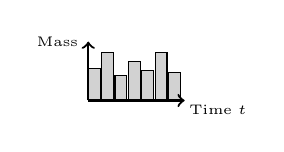
\begin{tikzpicture}[scale=0.34,baseline]
        \foreach \t/\h in {0/1.2,1/1.8,2/0.95,3/1.45,4/1.13,5/1.8,6/1.05}{
          \draw[fill=gray!35] (\t*0.50,0) rectangle ++(0.44,\h);
        }
        \draw[->,thick] (0,0) -- (3.6,0) node[below right=-2pt] {\tiny Time $t$};
        \draw[->,thick] (0,0) -- (0,2.2) node[left] {\tiny Mass};
      \end{tikzpicture}
    };
    \node[below=4pt of mass] {\scriptsize daily mass series $M(t)$};
    
    % ----------------------------------------------------------
    % (5) entropy scores
    % ----------------------------------------------------------
    \node[scalarbox,right=of mass] (entropy)
      {\Large$\displaystyle\frac{H\!\bigl(M_{\text{norm}}\bigr)}{H_{\text{unif}}}$};
    \node[below=4pt of entropy,align=center]
      {\scriptsize 5 normalised entropy scores\\[-1pt]\scriptsize (one for each fuzzy cluster)};
    
    % ----------------------------------------------------------
    % arrows
    % ----------------------------------------------------------
    \draw[arrow] (meanvec.east) -- ++(1.0,0) -- (Vsmall.west)
      node[process,above,yshift=12pt,pos=0]{fuzzy\,c-means\\clustering};
    
    \draw[arrow] (Vlarge.east) -- ++(0.9,0) -- (active.west)
      node[process,above,yshift=12pt,pos=0.35]{\textbf{for each of the 5}\\membership vectors select\\active interventions\\for each day};
    
    \draw[arrow] (active.east) -- (mass.west)
      node[process,above,yshift=12pt,pos=0.5]{aggregate\\per day};
    
    \draw[arrow] (mass.east) -- (entropy.west)
      node[process,above,yshift=12pt,pos=0.5]{normalise by\\total mass};
    
    \end{tikzpicture}%
      }
  
      % A little breathing room between rows (optional)
      \vspace{1.5ex}
  
      % Second row ──────────────────────────────────────────────
      \adjustbox{max width=0.9\linewidth, center}{%
        
\begin{tikzpicture}[node distance=3.4cm and 2.3cm]

% ----------------------------------------------------------
% (1) crisp 5×5 distance matrix
% ----------------------------------------------------------
\node[matrixbox] (crisp) {
  \begin{tikzpicture}[scale=0.55,baseline]
    \foreach \i in {0,...,5}{
      \draw[very thin,gray!65] (0,\i) -- (5,\i);
      \draw[very thin,gray!65] (\i,0) -- (\i,5);
    }
  \end{tikzpicture}
};
\node[below=4pt of crisp] {\scriptsize Crisp distance matrix $\mathbf{D}$};

% ----------------------------------------------------------
% (2) stack of 5 membership matrices (3×3 each)
% ----------------------------------------------------------
\foreach \name/\x/\col in {close/0/closec,midclose/1/midclosec,mid/2/midc,midfar/3/midfarc,far/4/farc}{
  \node[fuzzymatrix=\col,right=of crisp,xshift={(\x)*0.34cm-0.34cm}] (M\name){
    \begin{tikzpicture}[scale=0.29]
      \foreach \i in {0,...,3}{
        \draw[very thin,white] (0,\i) -- (3,\i);
        \draw[very thin,white] (\i,0) -- (\i,3);
      }
    \end{tikzpicture}
  };
}
\node[below=4pt of Mmid,align=center]
  {\scriptsize 5 fuzzy membership matrices\\[-1pt]\scriptsize (one per linguistic term)};

% ----------------------------------------------------------
% (3) 3×3 active-day matrix with blue shade & stair
% ----------------------------------------------------------
\node[matrixbox,right=of Mmidfar,xshift=1.1cm] (pairs) {
  \begin{tikzpicture}[scale=0.65,baseline]
    % 3×3 grid
    \foreach \i in {0,...,3}{
      \draw[very thin,gray!65] (0,\i) -- (3,\i);
      \draw[very thin,gray!65] (\i,0) -- (\i,3);
    }
    % shade cells strictly above diagonal
    \foreach \row/\col in {0/1,0/2,1/2}{
      \fill[closec!28] (\col,3-\row-1) rectangle ++(1,1);
    }
    % orange stair (border directly above diagonal) –– **top segment removed**
    \draw[midfarc,ultra thick]
      (1,3) -- (1,2) -- (2,2) -- (2,1) -- (3,1);
  \end{tikzpicture}
};
\node[below=5pt of pairs,align=center]
  {\scriptsize unique pairs (upper-triangular)\\[-1pt]\scriptsize of \emph{active-day} matrix};

% ----------------------------------------------------------
% (4) daily mass series
% ----------------------------------------------------------
\node[matrixbox,right=of pairs] (mass) {
  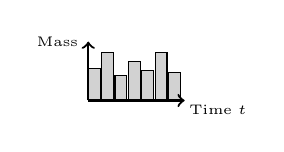
\begin{tikzpicture}[scale=0.34,baseline]
    \foreach \t/\h in {0/1.2,1/1.8,2/0.95,3/1.45,4/1.13,5/1.8,6/1.05}{
      \draw[fill=gray!35] (\t*0.50,0) rectangle ++(0.44,\h);
    }
    \draw[->,thick] (0,0) -- (3.6,0) node[below right=-2pt] {\tiny Time $t$};
    \draw[->,thick] (0,0) -- (0,2.2) node[left] {\tiny Mass};
  \end{tikzpicture}
};
\node[below=4pt of mass] {\scriptsize daily mass series $M(t)$};

% ----------------------------------------------------------
% (5) entropy scores
% ----------------------------------------------------------
\node[scalarbox,right=of mass] (entropy)
  {\Large$-\displaystyle\frac{H\!\bigl(M_{\text{norm}}\bigr)}{H_{\text{unif}}}$};
\node[below=4pt of entropy,align=center]
  {\scriptsize 5 normalised entropy scores\\[-1pt]\scriptsize (one for each fuzzy term)};

% ----------------------------------------------------------
% arrows
% ----------------------------------------------------------
% Arrow 1: crisp → membership  (slightly longer, label higher)
\draw[arrow] (crisp.east) -- ++(1.0,0) -- (Mclose.west)
  node[process,above,yshift=12pt,pos=0]{apply\\linguistic\\ variable};

% Arrow 2: membership → pairs
\draw[arrow] (Mmidfar.east) -- ++(0.9,0) -- (pairs.west)
  node[process,above,yshift=12pt,pos=0.4]%
       {extract active interventions\\(submatrix)\par\textbf{for each of the 5}\\membership matrices};

% Arrow 3: pairs → mass
\draw[arrow] (pairs.east) -- (mass.west)
  node[process,above,yshift=12pt,pos=0.5]{aggregate\\per day};

% Arrow 4: mass → entropy
\draw[arrow] (mass.east) -- (entropy.west)
  node[process,above,yshift=12pt,pos=0.5]{normalise by\\total mass};

\end{tikzpicture}%
      }
  
      % More breathing room (optional)
      \vspace{1.5ex}
  
      % Third row ───────────────────────────────────────────────
      \adjustbox{max width=0.9\linewidth, center}{%
        \begin{tikzpicture}[node distance=3.4cm and 2.3cm]

    % ----------------------------------------------------------
    % (1) crisp distance matrix  --- interventions × parks
    % ----------------------------------------------------------
    \node[matrixbox] (crisp) {
      \begin{tikzpicture}[scale=0.55,baseline]
        % 5 rows (interventions) × 4 cols (parks)
        \foreach \i in {0,...,5}{
          \draw[very thin,gray!65] (0,\i) -- (4,\i);
        }
        \foreach \j in {0,...,4}{
          \draw[very thin,gray!65] (\j,0) -- (\j,5);
        }
      \end{tikzpicture}
    };
    \node[below=4pt of crisp,align=center]
      {\scriptsize Crisp distance matrix $\mathbf{D}$\\[-1pt]\scriptsize (interventions $\times$ parks)};
    
    % ----------------------------------------------------------
    % (2) stack of 5 membership matrices (5×4 each)
    % ----------------------------------------------------------
    \foreach \name/\x/\col in {close/0/closec,midclose/1/midclosec,mid/2/midc,midfar/3/midfarc,far/4/farc}{
      \node[fuzzymatrix=\col,right=of crisp,xshift={(\x)*0.34cm-0.34cm}] (M\name){
        \begin{tikzpicture}[scale=0.23] % 5×4 tiny grid
          \foreach \i in {0,...,5}{
            \draw[very thin,white] (0,\i) -- (4,\i);
          }
          \foreach \j in {0,...,4}{
            \draw[very thin,white] (\j,0) -- (\j,5);
          }
        \end{tikzpicture}
      };
    }
    \node[below=4pt of Mmid,align=center]
      {\scriptsize 5 fuzzy membership matrices\\[-1pt]\scriptsize (one per linguistic term)};
    
    % ----------------------------------------------------------
    % (3) aggregated membership vector (t-conorm)
    % ----------------------------------------------------------
    \node[matrixbox,right=of Mmidfar,xshift=1.1cm] (agg) {
      \begin{tikzpicture}[scale=0.65,baseline]
        % 5×1 column vector grid
        \foreach \i in {0,...,5}{
          \draw[very thin,gray!65] (0,\i) -- (1,\i);
        }
        \draw[very thin,gray!65] (0,0) -- (0,5);
        \draw[very thin,gray!65] (1,0) -- (1,5);
        % shade only the 1st, 3rd and 5th cells
        \foreach \y in {0,2,4}{
          \fill[closec!28] (0,\y) rectangle ++(1,1);
        }
      \end{tikzpicture}
    };
    \node[below=5pt of agg,align=center]
      {\scriptsize aggregated memberships\\[-1pt]\scriptsize per intervention. In blue,\\
      \scriptsize active interventions};
    
    % ----------------------------------------------------------
    % (4) daily mass series
    % ----------------------------------------------------------
    \node[matrixbox,right=of agg] (mass) {
      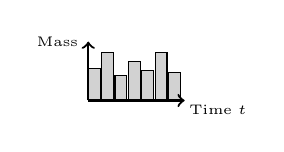
\begin{tikzpicture}[scale=0.34,baseline]
        \foreach \t/\h in {0/1.2,1/1.8,2/0.95,3/1.45,4/1.13,5/1.8,6/1.05}{
          \draw[fill=gray!35] (\t*0.50,0) rectangle ++(0.44,\h);
        }
        \draw[->,thick] (0,0) -- (3.6,0) node[below right=-2pt] {\tiny Time $t$};
        \draw[->,thick] (0,0) -- (0,2.2) node[left] {\tiny Mass};
      \end{tikzpicture}
    };
    \node[below=4pt of mass] {\scriptsize daily mass series $M(t)$};
    
    % ----------------------------------------------------------
    % (5) entropy scores
    % ----------------------------------------------------------
    \node[scalarbox,right=of mass] (entropy)
      {\Large$\displaystyle\frac{H\!\bigl(M_{\text{norm}}\bigr)}{H_{\text{unif}}}$};
    \node[below=4pt of entropy,align=center]
      {\scriptsize 5 normalised entropy scores\\[-1pt]\scriptsize (one for each fuzzy term)};
    
    % ----------------------------------------------------------
    % arrows
    % ----------------------------------------------------------
    \draw[arrow] (crisp.east) -- ++(1.0,0) -- (Mclose.west)
      node[process,above,yshift=12pt,pos=0]{apply\\linguistic\\ variable};
    
    \draw[arrow] (Mmidfar.east) -- ++(0.9,0) -- (agg.west)
      node[process,above,yshift=12pt,pos=0.4]%
           {row-wise aggregation\\(T-conorm)\par\textbf{for each of the 5}\\membership matrices};
    
    \draw[arrow] (agg.east) -- (mass.west)
      node[process,above,yshift=12pt,pos=0.5]{aggregate\\per day};
    
    \draw[arrow] (mass.east) -- (entropy.west)
      node[process,above,yshift=12pt,pos=0.5]{normalise by\\total mass};
    
    \end{tikzpicture}%
      }
  
    \end{adjustwidth}
  
    \caption{Overview of fuzzy attribute pipelines: risk/size (top), closeness (middle) and environmental
             impact (bottom) diagrams.}
    \label{fig:risk-size_closeness_envimpact}
  \end{figure}

\thispagestyle{empty}
  \restoregeometry          % margin settings back to normal
\clearpage   


\clearpage
\newgeometry{bottom=0.6cm}
\begin{sidewaystable}[!ht]
\thispagestyle{empty}
\centering
\scriptsize
\setlength\tabcolsep{3pt}
\renewcommand{\arraystretch}{1.5}
\resizebox{1.12\textheight}{!}{

\begin{tabular}{|l|c|ccccc|ccccc|ccccc|ccccc|ccc|}
\hline

\multirow{2}{*}{\rule{0pt}{2.3ex}\textbf{Solutions}} &
\multirow{2}{*}{\rule{0pt}{2.3ex}\shortstack{\textbf{Highest}\\\textbf{Concurrency}}} &
\multicolumn{5}{c|}{\textbf{Size Concurrency}} &
\multicolumn{5}{c|}{\textbf{Risk Concurrency}} &
\multicolumn{5}{c|}{\textbf{Closeness Concurrency}} &
\multicolumn{5}{c|}{\textbf{Environmental-Impact Concurrency}} &
\multicolumn{3}{c|}{\textbf{Seasonality}} \\[2pt]
& & \cellcolor{SizeBase!10}small & \cellcolor{SizeBase!20}mid-small & \cellcolor{SizeBase!30}mid & \cellcolor{SizeBase!40}mid-large & \cellcolor{SizeBase!50}large & \cellcolor{RiskBase!10}low & \cellcolor{RiskBase!20}mid-low & \cellcolor{RiskBase!30}mid & \cellcolor{RiskBase!40}mid-high & \cellcolor{RiskBase!50}high & \cellcolor{CloseBase!10}close & \cellcolor{CloseBase!20}mid-close & \cellcolor{CloseBase!30}mid & \cellcolor{CloseBase!40}mid-far & \cellcolor{CloseBase!50}far & \cellcolor{EnvBase!10}low & \cellcolor{EnvBase!20}mid-low & \cellcolor{EnvBase!30}mid & \cellcolor{EnvBase!40}mid-high & \cellcolor{EnvBase!50}high & \cellcolor{Winter}Winter & \cellcolor{Summer}Summer & \cellcolor{Inter}Inter-season \\
\hline
T1\_D180\_S33 & 0.392 & \cellcolor{SizeBase!10}0.987 & \cellcolor{SizeBase!20}0.982 & \cellcolor{SizeBase!30}0.982 & \cellcolor{SizeBase!40}0.996 & \cellcolor{SizeBase!50}0.993 & \cellcolor{RiskBase!10}0.994 & \cellcolor{RiskBase!20}0.990 & \cellcolor{RiskBase!30}0.990 & \cellcolor{RiskBase!40}0.990 & \cellcolor{RiskBase!50}0.984 & \cellcolor{CloseBase!10}0.971 & \cellcolor{CloseBase!20}0.972 & \cellcolor{CloseBase!30}0.970 & \cellcolor{CloseBase!40}0.972 & \cellcolor{CloseBase!50}0.972 & \cellcolor{EnvBase!10}0.990 & \cellcolor{EnvBase!20}0.986 & \cellcolor{EnvBase!30}0.990 & \cellcolor{EnvBase!40}0.991 & \cellcolor{EnvBase!50}0.991 & \cellcolor{Winter}0.618 & \cellcolor{Summer}0.622 & \cellcolor{Inter}0.607 \\
T1\_D180\_S42 & 0.390 & \cellcolor{SizeBase!10}0.987 & \cellcolor{SizeBase!20}0.983 & \cellcolor{SizeBase!30}0.984 & \cellcolor{SizeBase!40}0.996 & \cellcolor{SizeBase!50}0.993 & \cellcolor{RiskBase!10}0.995 & \cellcolor{RiskBase!20}0.991 & \cellcolor{RiskBase!30}0.990 & \cellcolor{RiskBase!40}0.989 & \cellcolor{RiskBase!50}0.983 & \cellcolor{CloseBase!10}0.967 & \cellcolor{CloseBase!20}0.973 & \cellcolor{CloseBase!30}0.971 & \cellcolor{CloseBase!40}0.972 & \cellcolor{CloseBase!50}0.972 & \cellcolor{EnvBase!10}0.990 & \cellcolor{EnvBase!20}0.985 & \cellcolor{EnvBase!30}0.990 & \cellcolor{EnvBase!40}0.991 & \cellcolor{EnvBase!50}0.991 & \cellcolor{Winter}0.624 & \cellcolor{Summer}0.622 & \cellcolor{Inter}0.601 \\
T1\_D180\_S73 & 0.386 & \cellcolor{SizeBase!10}0.986 & \cellcolor{SizeBase!20}0.982 & \cellcolor{SizeBase!30}0.985 & \cellcolor{SizeBase!40}0.996 & \cellcolor{SizeBase!50}0.992 & \cellcolor{RiskBase!10}0.993 & \cellcolor{RiskBase!20}0.990 & \cellcolor{RiskBase!30}0.990 & \cellcolor{RiskBase!40}0.990 & \cellcolor{RiskBase!50}0.983 & \cellcolor{CloseBase!10}0.975 & \cellcolor{CloseBase!20}0.973 & \cellcolor{CloseBase!30}0.970 & \cellcolor{CloseBase!40}0.971 & \cellcolor{CloseBase!50}0.972 & \cellcolor{EnvBase!10}0.988 & \cellcolor{EnvBase!20}0.985 & \cellcolor{EnvBase!30}0.989 & \cellcolor{EnvBase!40}0.990 & \cellcolor{EnvBase!50}0.991 & \cellcolor{Winter}0.610 & \cellcolor{Summer}0.628 & \cellcolor{Inter}0.597 \\
T1\_D300\_S33 & 0.378 & \cellcolor{SizeBase!10}0.986 & \cellcolor{SizeBase!20}0.976 & \cellcolor{SizeBase!30}0.980 & \cellcolor{SizeBase!40}0.996 & \cellcolor{SizeBase!50}0.993 & \cellcolor{RiskBase!10}0.994 & \cellcolor{RiskBase!20}0.990 & \cellcolor{RiskBase!30}0.988 & \cellcolor{RiskBase!40}0.989 & \cellcolor{RiskBase!50}0.983 & \cellcolor{CloseBase!10}0.970 & \cellcolor{CloseBase!20}0.972 & \cellcolor{CloseBase!30}0.969 & \cellcolor{CloseBase!40}0.969 & \cellcolor{CloseBase!50}0.970 & \cellcolor{EnvBase!10}0.990 & \cellcolor{EnvBase!20}0.982 & \cellcolor{EnvBase!30}0.989 & \cellcolor{EnvBase!40}0.989 & \cellcolor{EnvBase!50}0.990 & \cellcolor{Winter}0.620 & \cellcolor{Summer}0.622 & \cellcolor{Inter}0.622 \\
T1\_D300\_S42 & 0.382 & \cellcolor{SizeBase!10}0.986 & \cellcolor{SizeBase!20}0.977 & \cellcolor{SizeBase!30}0.980 & \cellcolor{SizeBase!40}0.996 & \cellcolor{SizeBase!50}0.993 & \cellcolor{RiskBase!10}0.994 & \cellcolor{RiskBase!20}0.989 & \cellcolor{RiskBase!30}0.988 & \cellcolor{RiskBase!40}0.990 & \cellcolor{RiskBase!50}0.983 & \cellcolor{CloseBase!10}0.968 & \cellcolor{CloseBase!20}0.970 & \cellcolor{CloseBase!30}0.969 & \cellcolor{CloseBase!40}0.969 & \cellcolor{CloseBase!50}0.971 & \cellcolor{EnvBase!10}0.990 & \cellcolor{EnvBase!20}0.983 & \cellcolor{EnvBase!30}0.990 & \cellcolor{EnvBase!40}0.989 & \cellcolor{EnvBase!50}0.990 & \cellcolor{Winter}0.614 & \cellcolor{Summer}0.626 & \cellcolor{Inter}0.616 \\
T1\_D300\_S73 & 0.384 & \cellcolor{SizeBase!10}0.985 & \cellcolor{SizeBase!20}0.977 & \cellcolor{SizeBase!30}0.987 & \cellcolor{SizeBase!40}0.996 & \cellcolor{SizeBase!50}0.993 & \cellcolor{RiskBase!10}0.993 & \cellcolor{RiskBase!20}0.991 & \cellcolor{RiskBase!30}0.988 & \cellcolor{RiskBase!40}0.991 & \cellcolor{RiskBase!50}0.980 & \cellcolor{CloseBase!10}0.965 & \cellcolor{CloseBase!20}0.975 & \cellcolor{CloseBase!30}0.969 & \cellcolor{CloseBase!40}0.970 & \cellcolor{CloseBase!50}0.970 & \cellcolor{EnvBase!10}0.989 & \cellcolor{EnvBase!20}0.986 & \cellcolor{EnvBase!30}0.990 & \cellcolor{EnvBase!40}0.990 & \cellcolor{EnvBase!50}0.990 & \cellcolor{Winter}0.610 & \cellcolor{Summer}0.630 & \cellcolor{Inter}0.597 \\
T1\_D500\_S33 & 0.401 & \cellcolor{SizeBase!10}0.985 & \cellcolor{SizeBase!20}0.973 & \cellcolor{SizeBase!30}0.983 & \cellcolor{SizeBase!40}0.996 & \cellcolor{SizeBase!50}0.993 & \cellcolor{RiskBase!10}0.996 & \cellcolor{RiskBase!20}0.986 & \cellcolor{RiskBase!30}0.989 & \cellcolor{RiskBase!40}0.989 & \cellcolor{RiskBase!50}0.984 & \cellcolor{CloseBase!10}0.968 & \cellcolor{CloseBase!20}0.971 & \cellcolor{CloseBase!30}0.966 & \cellcolor{CloseBase!40}0.968 & \cellcolor{CloseBase!50}0.969 & \cellcolor{EnvBase!10}0.990 & \cellcolor{EnvBase!20}0.982 & \cellcolor{EnvBase!30}0.990 & \cellcolor{EnvBase!40}0.989 & \cellcolor{EnvBase!50}0.990 & \cellcolor{Winter}0.610 & \cellcolor{Summer}0.633 & \cellcolor{Inter}0.597 \\
T1\_D500\_S42 & 0.399 & \cellcolor{SizeBase!10}0.985 & \cellcolor{SizeBase!20}0.972 & \cellcolor{SizeBase!30}0.983 & \cellcolor{SizeBase!40}0.996 & \cellcolor{SizeBase!50}0.993 & \cellcolor{RiskBase!10}0.995 & \cellcolor{RiskBase!20}0.987 & \cellcolor{RiskBase!30}0.988 & \cellcolor{RiskBase!40}0.989 & \cellcolor{RiskBase!50}0.984 & \cellcolor{CloseBase!10}0.968 & \cellcolor{CloseBase!20}0.972 & \cellcolor{CloseBase!30}0.967 & \cellcolor{CloseBase!40}0.967 & \cellcolor{CloseBase!50}0.968 & \cellcolor{EnvBase!10}0.989 & \cellcolor{EnvBase!20}0.984 & \cellcolor{EnvBase!30}0.991 & \cellcolor{EnvBase!40}0.989 & \cellcolor{EnvBase!50}0.989 & \cellcolor{Winter}0.608 & \cellcolor{Summer}0.633 & \cellcolor{Inter}0.597 \\
T1\_D500\_S73 & 0.395 & \cellcolor{SizeBase!10}0.986 & \cellcolor{SizeBase!20}0.972 & \cellcolor{SizeBase!30}0.983 & \cellcolor{SizeBase!40}0.996 & \cellcolor{SizeBase!50}0.993 & \cellcolor{RiskBase!10}0.994 & \cellcolor{RiskBase!20}0.987 & \cellcolor{RiskBase!30}0.988 & \cellcolor{RiskBase!40}0.989 & \cellcolor{RiskBase!50}0.983 & \cellcolor{CloseBase!10}0.965 & \cellcolor{CloseBase!20}0.971 & \cellcolor{CloseBase!30}0.966 & \cellcolor{CloseBase!40}0.968 & \cellcolor{CloseBase!50}0.969 & \cellcolor{EnvBase!10}0.990 & \cellcolor{EnvBase!20}0.984 & \cellcolor{EnvBase!30}0.991 & \cellcolor{EnvBase!40}0.989 & \cellcolor{EnvBase!50}0.990 & \cellcolor{Winter}0.608 & \cellcolor{Summer}0.633 & \cellcolor{Inter}0.603 \\
T1\_D700\_S33 & 0.403 & \cellcolor{SizeBase!10}0.985 & \cellcolor{SizeBase!20}0.974 & \cellcolor{SizeBase!30}0.984 & \cellcolor{SizeBase!40}0.996 & \cellcolor{SizeBase!50}0.992 & \cellcolor{RiskBase!10}0.996 & \cellcolor{RiskBase!20}0.987 & \cellcolor{RiskBase!30}0.989 & \cellcolor{RiskBase!40}0.989 & \cellcolor{RiskBase!50}0.983 & \cellcolor{CloseBase!10}0.968 & \cellcolor{CloseBase!20}0.971 & \cellcolor{CloseBase!30}0.966 & \cellcolor{CloseBase!40}0.968 & \cellcolor{CloseBase!50}0.969 & \cellcolor{EnvBase!10}0.990 & \cellcolor{EnvBase!20}0.985 & \cellcolor{EnvBase!30}0.990 & \cellcolor{EnvBase!40}0.989 & \cellcolor{EnvBase!50}0.990 & \cellcolor{Winter}0.610 & \cellcolor{Summer}0.630 & \cellcolor{Inter}0.607 \\
T1\_D700\_S42 & 0.393 & \cellcolor{SizeBase!10}0.985 & \cellcolor{SizeBase!20}0.974 & \cellcolor{SizeBase!30}0.984 & \cellcolor{SizeBase!40}0.996 & \cellcolor{SizeBase!50}0.992 & \cellcolor{RiskBase!10}0.996 & \cellcolor{RiskBase!20}0.987 & \cellcolor{RiskBase!30}0.988 & \cellcolor{RiskBase!40}0.989 & \cellcolor{RiskBase!50}0.983 & \cellcolor{CloseBase!10}0.971 & \cellcolor{CloseBase!20}0.972 & \cellcolor{CloseBase!30}0.967 & \cellcolor{CloseBase!40}0.968 & \cellcolor{CloseBase!50}0.969 & \cellcolor{EnvBase!10}0.989 & \cellcolor{EnvBase!20}0.984 & \cellcolor{EnvBase!30}0.991 & \cellcolor{EnvBase!40}0.989 & \cellcolor{EnvBase!50}0.990 & \cellcolor{Winter}0.610 & \cellcolor{Summer}0.631 & \cellcolor{Inter}0.595 \\
T1\_D700\_S73 & 0.390 & \cellcolor{SizeBase!10}0.985 & \cellcolor{SizeBase!20}0.973 & \cellcolor{SizeBase!30}0.984 & \cellcolor{SizeBase!40}0.996 & \cellcolor{SizeBase!50}0.992 & \cellcolor{RiskBase!10}0.995 & \cellcolor{RiskBase!20}0.987 & \cellcolor{RiskBase!30}0.989 & \cellcolor{RiskBase!40}0.989 & \cellcolor{RiskBase!50}0.985 & \cellcolor{CloseBase!10}0.969 & \cellcolor{CloseBase!20}0.971 & \cellcolor{CloseBase!30}0.967 & \cellcolor{CloseBase!40}0.968 & \cellcolor{CloseBase!50}0.969 & \cellcolor{EnvBase!10}0.990 & \cellcolor{EnvBase!20}0.985 & \cellcolor{EnvBase!30}0.991 & \cellcolor{EnvBase!40}0.989 & \cellcolor{EnvBase!50}0.990 & \cellcolor{Winter}0.610 & \cellcolor{Summer}0.630 & \cellcolor{Inter}0.608 \\
T1\_D900\_S33 & 0.388 & \cellcolor{SizeBase!10}0.983 & \cellcolor{SizeBase!20}0.976 & \cellcolor{SizeBase!30}0.984 & \cellcolor{SizeBase!40}0.996 & \cellcolor{SizeBase!50}0.993 & \cellcolor{RiskBase!10}0.995 & \cellcolor{RiskBase!20}0.986 & \cellcolor{RiskBase!30}0.987 & \cellcolor{RiskBase!40}0.989 & \cellcolor{RiskBase!50}0.986 & \cellcolor{CloseBase!10}0.965 & \cellcolor{CloseBase!20}0.971 & \cellcolor{CloseBase!30}0.966 & \cellcolor{CloseBase!40}0.967 & \cellcolor{CloseBase!50}0.968 & \cellcolor{EnvBase!10}0.989 & \cellcolor{EnvBase!20}0.982 & \cellcolor{EnvBase!30}0.990 & \cellcolor{EnvBase!40}0.988 & \cellcolor{EnvBase!50}0.989 & \cellcolor{Winter}0.601 & \cellcolor{Summer}0.641 & \cellcolor{Inter}0.605 \\
T1\_D900\_S42 & 0.395 & \cellcolor{SizeBase!10}0.985 & \cellcolor{SizeBase!20}0.973 & \cellcolor{SizeBase!30}0.985 & \cellcolor{SizeBase!40}0.996 & \cellcolor{SizeBase!50}0.992 & \cellcolor{RiskBase!10}0.996 & \cellcolor{RiskBase!20}0.986 & \cellcolor{RiskBase!30}0.988 & \cellcolor{RiskBase!40}0.989 & \cellcolor{RiskBase!50}0.984 & \cellcolor{CloseBase!10}0.961 & \cellcolor{CloseBase!20}0.971 & \cellcolor{CloseBase!30}0.966 & \cellcolor{CloseBase!40}0.967 & \cellcolor{CloseBase!50}0.968 & \cellcolor{EnvBase!10}0.990 & \cellcolor{EnvBase!20}0.983 & \cellcolor{EnvBase!30}0.990 & \cellcolor{EnvBase!40}0.989 & \cellcolor{EnvBase!50}0.990 & \cellcolor{Winter}0.607 & \cellcolor{Summer}0.633 & \cellcolor{Inter}0.608 \\
T1\_D900\_S73 & 0.395 & \cellcolor{SizeBase!10}0.985 & \cellcolor{SizeBase!20}0.975 & \cellcolor{SizeBase!30}0.984 & \cellcolor{SizeBase!40}0.996 & \cellcolor{SizeBase!50}0.993 & \cellcolor{RiskBase!10}0.995 & \cellcolor{RiskBase!20}0.986 & \cellcolor{RiskBase!30}0.990 & \cellcolor{RiskBase!40}0.990 & \cellcolor{RiskBase!50}0.985 & \cellcolor{CloseBase!10}0.969 & \cellcolor{CloseBase!20}0.973 & \cellcolor{CloseBase!30}0.967 & \cellcolor{CloseBase!40}0.968 & \cellcolor{CloseBase!50}0.969 & \cellcolor{EnvBase!10}0.989 & \cellcolor{EnvBase!20}0.985 & \cellcolor{EnvBase!30}0.991 & \cellcolor{EnvBase!40}0.989 & \cellcolor{EnvBase!50}0.990 & \cellcolor{Winter}0.603 & \cellcolor{Summer}0.635 & \cellcolor{Inter}0.595 \\
T3\_D180\_S33 & 0.401 & \cellcolor{SizeBase!10}0.985 & \cellcolor{SizeBase!20}0.972 & \cellcolor{SizeBase!30}0.985 & \cellcolor{SizeBase!40}0.996 & \cellcolor{SizeBase!50}0.991 & \cellcolor{RiskBase!10}0.994 & \cellcolor{RiskBase!20}0.985 & \cellcolor{RiskBase!30}0.989 & \cellcolor{RiskBase!40}0.990 & \cellcolor{RiskBase!50}0.983 & \cellcolor{CloseBase!10}0.962 & \cellcolor{CloseBase!20}0.971 & \cellcolor{CloseBase!30}0.967 & \cellcolor{CloseBase!40}0.967 & \cellcolor{CloseBase!50}0.969 & \cellcolor{EnvBase!10}0.990 & \cellcolor{EnvBase!20}0.983 & \cellcolor{EnvBase!30}0.989 & \cellcolor{EnvBase!40}0.989 & \cellcolor{EnvBase!50}0.990 & \cellcolor{Winter}0.605 & \cellcolor{Summer}0.637 & \cellcolor{Inter}0.605 \\
T3\_D180\_S42 & 0.393 & \cellcolor{SizeBase!10}0.985 & \cellcolor{SizeBase!20}0.976 & \cellcolor{SizeBase!30}0.984 & \cellcolor{SizeBase!40}0.996 & \cellcolor{SizeBase!50}0.993 & \cellcolor{RiskBase!10}0.994 & \cellcolor{RiskBase!20}0.987 & \cellcolor{RiskBase!30}0.989 & \cellcolor{RiskBase!40}0.991 & \cellcolor{RiskBase!50}0.983 & \cellcolor{CloseBase!10}0.963 & \cellcolor{CloseBase!20}0.970 & \cellcolor{CloseBase!30}0.968 & \cellcolor{CloseBase!40}0.969 & \cellcolor{CloseBase!50}0.970 & \cellcolor{EnvBase!10}0.991 & \cellcolor{EnvBase!20}0.982 & \cellcolor{EnvBase!30}0.990 & \cellcolor{EnvBase!40}0.989 & \cellcolor{EnvBase!50}0.990 & \cellcolor{Winter}0.608 & \cellcolor{Summer}0.631 & \cellcolor{Inter}0.595 \\
T3\_D180\_S73 & 0.405 & \cellcolor{SizeBase!10}0.984 & \cellcolor{SizeBase!20}0.976 & \cellcolor{SizeBase!30}0.985 & \cellcolor{SizeBase!40}0.996 & \cellcolor{SizeBase!50}0.993 & \cellcolor{RiskBase!10}0.994 & \cellcolor{RiskBase!20}0.987 & \cellcolor{RiskBase!30}0.989 & \cellcolor{RiskBase!40}0.990 & \cellcolor{RiskBase!50}0.982 & \cellcolor{CloseBase!10}0.963 & \cellcolor{CloseBase!20}0.972 & \cellcolor{CloseBase!30}0.967 & \cellcolor{CloseBase!40}0.968 & \cellcolor{CloseBase!50}0.969 & \cellcolor{EnvBase!10}0.990 & \cellcolor{EnvBase!20}0.984 & \cellcolor{EnvBase!30}0.990 & \cellcolor{EnvBase!40}0.989 & \cellcolor{EnvBase!50}0.990 & \cellcolor{Winter}0.599 & \cellcolor{Summer}0.635 & \cellcolor{Inter}0.597 \\
T3\_D300\_S33 & 0.392 & \cellcolor{SizeBase!10}0.984 & \cellcolor{SizeBase!20}0.976 & \cellcolor{SizeBase!30}0.985 & \cellcolor{SizeBase!40}0.996 & \cellcolor{SizeBase!50}0.993 & \cellcolor{RiskBase!10}0.995 & \cellcolor{RiskBase!20}0.986 & \cellcolor{RiskBase!30}0.988 & \cellcolor{RiskBase!40}0.989 & \cellcolor{RiskBase!50}0.986 & \cellcolor{CloseBase!10}0.968 & \cellcolor{CloseBase!20}0.972 & \cellcolor{CloseBase!30}0.968 & \cellcolor{CloseBase!40}0.968 & \cellcolor{CloseBase!50}0.969 & \cellcolor{EnvBase!10}0.991 & \cellcolor{EnvBase!20}0.981 & \cellcolor{EnvBase!30}0.989 & \cellcolor{EnvBase!40}0.989 & \cellcolor{EnvBase!50}0.990 & \cellcolor{Winter}0.624 & \cellcolor{Summer}0.618 & \cellcolor{Inter}0.616 \\
T3\_D300\_S42 & 0.395 & \cellcolor{SizeBase!10}0.985 & \cellcolor{SizeBase!20}0.975 & \cellcolor{SizeBase!30}0.986 & \cellcolor{SizeBase!40}0.996 & \cellcolor{SizeBase!50}0.993 & \cellcolor{RiskBase!10}0.993 & \cellcolor{RiskBase!20}0.988 & \cellcolor{RiskBase!30}0.990 & \cellcolor{RiskBase!40}0.990 & \cellcolor{RiskBase!50}0.983 & \cellcolor{CloseBase!10}0.966 & \cellcolor{CloseBase!20}0.973 & \cellcolor{CloseBase!30}0.968 & \cellcolor{CloseBase!40}0.968 & \cellcolor{CloseBase!50}0.970 & \cellcolor{EnvBase!10}0.990 & \cellcolor{EnvBase!20}0.983 & \cellcolor{EnvBase!30}0.990 & \cellcolor{EnvBase!40}0.989 & \cellcolor{EnvBase!50}0.990 & \cellcolor{Winter}0.597 & \cellcolor{Summer}0.639 & \cellcolor{Inter}0.610 \\
T3\_D300\_S73 & 0.401 & \cellcolor{SizeBase!10}0.985 & \cellcolor{SizeBase!20}0.972 & \cellcolor{SizeBase!30}0.985 & \cellcolor{SizeBase!40}0.996 & \cellcolor{SizeBase!50}0.993 & \cellcolor{RiskBase!10}0.993 & \cellcolor{RiskBase!20}0.987 & \cellcolor{RiskBase!30}0.989 & \cellcolor{RiskBase!40}0.990 & \cellcolor{RiskBase!50}0.983 & \cellcolor{CloseBase!10}0.959 & \cellcolor{CloseBase!20}0.970 & \cellcolor{CloseBase!30}0.969 & \cellcolor{CloseBase!40}0.969 & \cellcolor{CloseBase!50}0.969 & \cellcolor{EnvBase!10}0.989 & \cellcolor{EnvBase!20}0.983 & \cellcolor{EnvBase!30}0.990 & \cellcolor{EnvBase!40}0.989 & \cellcolor{EnvBase!50}0.990 & \cellcolor{Winter}0.608 & \cellcolor{Summer}0.628 & \cellcolor{Inter}0.599 \\
T3\_D500\_S33 & 0.399 & \cellcolor{SizeBase!10}0.984 & \cellcolor{SizeBase!20}0.977 & \cellcolor{SizeBase!30}0.986 & \cellcolor{SizeBase!40}0.996 & \cellcolor{SizeBase!50}0.994 & \cellcolor{RiskBase!10}0.995 & \cellcolor{RiskBase!20}0.988 & \cellcolor{RiskBase!30}0.989 & \cellcolor{RiskBase!40}0.990 & \cellcolor{RiskBase!50}0.982 & \cellcolor{CloseBase!10}0.965 & \cellcolor{CloseBase!20}0.974 & \cellcolor{CloseBase!30}0.967 & \cellcolor{CloseBase!40}0.968 & \cellcolor{CloseBase!50}0.970 & \cellcolor{EnvBase!10}0.992 & \cellcolor{EnvBase!20}0.982 & \cellcolor{EnvBase!30}0.989 & \cellcolor{EnvBase!40}0.989 & \cellcolor{EnvBase!50}0.990 & \cellcolor{Winter}0.605 & \cellcolor{Summer}0.639 & \cellcolor{Inter}0.601 \\
T3\_D500\_S42 & 0.395 & \cellcolor{SizeBase!10}0.985 & \cellcolor{SizeBase!20}0.974 & \cellcolor{SizeBase!30}0.986 & \cellcolor{SizeBase!40}0.996 & \cellcolor{SizeBase!50}0.994 & \cellcolor{RiskBase!10}0.994 & \cellcolor{RiskBase!20}0.987 & \cellcolor{RiskBase!30}0.989 & \cellcolor{RiskBase!40}0.991 & \cellcolor{RiskBase!50}0.983 & \cellcolor{CloseBase!10}0.961 & \cellcolor{CloseBase!20}0.973 & \cellcolor{CloseBase!30}0.969 & \cellcolor{CloseBase!40}0.969 & \cellcolor{CloseBase!50}0.970 & \cellcolor{EnvBase!10}0.992 & \cellcolor{EnvBase!20}0.982 & \cellcolor{EnvBase!30}0.989 & \cellcolor{EnvBase!40}0.989 & \cellcolor{EnvBase!50}0.990 & \cellcolor{Winter}0.603 & \cellcolor{Summer}0.639 & \cellcolor{Inter}0.612 \\
T3\_D500\_S73 & 0.405 & \cellcolor{SizeBase!10}0.985 & \cellcolor{SizeBase!20}0.974 & \cellcolor{SizeBase!30}0.984 & \cellcolor{SizeBase!40}0.996 & \cellcolor{SizeBase!50}0.993 & \cellcolor{RiskBase!10}0.993 & \cellcolor{RiskBase!20}0.987 & \cellcolor{RiskBase!30}0.989 & \cellcolor{RiskBase!40}0.989 & \cellcolor{RiskBase!50}0.984 & \cellcolor{CloseBase!10}0.963 & \cellcolor{CloseBase!20}0.972 & \cellcolor{CloseBase!30}0.967 & \cellcolor{CloseBase!40}0.968 & \cellcolor{CloseBase!50}0.969 & \cellcolor{EnvBase!10}0.990 & \cellcolor{EnvBase!20}0.983 & \cellcolor{EnvBase!30}0.990 & \cellcolor{EnvBase!40}0.988 & \cellcolor{EnvBase!50}0.990 & \cellcolor{Winter}0.607 & \cellcolor{Summer}0.633 & \cellcolor{Inter}0.599 \\
T3\_D700\_S33 & 0.415 & \cellcolor{SizeBase!10}0.984 & \cellcolor{SizeBase!20}0.971 & \cellcolor{SizeBase!30}0.984 & \cellcolor{SizeBase!40}0.996 & \cellcolor{SizeBase!50}0.993 & \cellcolor{RiskBase!10}0.994 & \cellcolor{RiskBase!20}0.986 & \cellcolor{RiskBase!30}0.990 & \cellcolor{RiskBase!40}0.990 & \cellcolor{RiskBase!50}0.983 & \cellcolor{CloseBase!10}0.966 & \cellcolor{CloseBase!20}0.968 & \cellcolor{CloseBase!30}0.965 & \cellcolor{CloseBase!40}0.966 & \cellcolor{CloseBase!50}0.968 & \cellcolor{EnvBase!10}0.990 & \cellcolor{EnvBase!20}0.980 & \cellcolor{EnvBase!30}0.989 & \cellcolor{EnvBase!40}0.989 & \cellcolor{EnvBase!50}0.990 & \cellcolor{Winter}0.605 & \cellcolor{Summer}0.637 & \cellcolor{Inter}0.583 \\
T3\_D700\_S42 & 0.395 & \cellcolor{SizeBase!10}0.986 & \cellcolor{SizeBase!20}0.976 & \cellcolor{SizeBase!30}0.986 & \cellcolor{SizeBase!40}0.996 & \cellcolor{SizeBase!50}0.994 & \cellcolor{RiskBase!10}0.993 & \cellcolor{RiskBase!20}0.987 & \cellcolor{RiskBase!30}0.990 & \cellcolor{RiskBase!40}0.991 & \cellcolor{RiskBase!50}0.984 & \cellcolor{CloseBase!10}0.966 & \cellcolor{CloseBase!20}0.973 & \cellcolor{CloseBase!30}0.968 & \cellcolor{CloseBase!40}0.968 & \cellcolor{CloseBase!50}0.970 & \cellcolor{EnvBase!10}0.992 & \cellcolor{EnvBase!20}0.982 & \cellcolor{EnvBase!30}0.990 & \cellcolor{EnvBase!40}0.989 & \cellcolor{EnvBase!50}0.990 & \cellcolor{Winter}0.605 & \cellcolor{Summer}0.633 & \cellcolor{Inter}0.607 \\
T3\_D700\_S73 & 0.401 & \cellcolor{SizeBase!10}0.986 & \cellcolor{SizeBase!20}0.972 & \cellcolor{SizeBase!30}0.983 & \cellcolor{SizeBase!40}0.996 & \cellcolor{SizeBase!50}0.994 & \cellcolor{RiskBase!10}0.996 & \cellcolor{RiskBase!20}0.985 & \cellcolor{RiskBase!30}0.989 & \cellcolor{RiskBase!40}0.990 & \cellcolor{RiskBase!50}0.983 & \cellcolor{CloseBase!10}0.963 & \cellcolor{CloseBase!20}0.970 & \cellcolor{CloseBase!30}0.967 & \cellcolor{CloseBase!40}0.968 & \cellcolor{CloseBase!50}0.969 & \cellcolor{EnvBase!10}0.991 & \cellcolor{EnvBase!20}0.979 & \cellcolor{EnvBase!30}0.989 & \cellcolor{EnvBase!40}0.989 & \cellcolor{EnvBase!50}0.990 & \cellcolor{Winter}0.608 & \cellcolor{Summer}0.630 & \cellcolor{Inter}0.612 \\
T3\_D900\_S33 & 0.403 & \cellcolor{SizeBase!10}0.985 & \cellcolor{SizeBase!20}0.971 & \cellcolor{SizeBase!30}0.984 & \cellcolor{SizeBase!40}0.996 & \cellcolor{SizeBase!50}0.993 & \cellcolor{RiskBase!10}0.995 & \cellcolor{RiskBase!20}0.986 & \cellcolor{RiskBase!30}0.988 & \cellcolor{RiskBase!40}0.992 & \cellcolor{RiskBase!50}0.984 & \cellcolor{CloseBase!10}0.959 & \cellcolor{CloseBase!20}0.973 & \cellcolor{CloseBase!30}0.968 & \cellcolor{CloseBase!40}0.968 & \cellcolor{CloseBase!50}0.970 & \cellcolor{EnvBase!10}0.991 & \cellcolor{EnvBase!20}0.982 & \cellcolor{EnvBase!30}0.989 & \cellcolor{EnvBase!40}0.989 & \cellcolor{EnvBase!50}0.990 & \cellcolor{Winter}0.603 & \cellcolor{Summer}0.641 & \cellcolor{Inter}0.595 \\
T3\_D900\_S42 & 0.393 & \cellcolor{SizeBase!10}0.985 & \cellcolor{SizeBase!20}0.976 & \cellcolor{SizeBase!30}0.986 & \cellcolor{SizeBase!40}0.996 & \cellcolor{SizeBase!50}0.993 & \cellcolor{RiskBase!10}0.993 & \cellcolor{RiskBase!20}0.987 & \cellcolor{RiskBase!30}0.990 & \cellcolor{RiskBase!40}0.990 & \cellcolor{RiskBase!50}0.984 & \cellcolor{CloseBase!10}0.965 & \cellcolor{CloseBase!20}0.973 & \cellcolor{CloseBase!30}0.968 & \cellcolor{CloseBase!40}0.969 & \cellcolor{CloseBase!50}0.970 & \cellcolor{EnvBase!10}0.990 & \cellcolor{EnvBase!20}0.983 & \cellcolor{EnvBase!30}0.990 & \cellcolor{EnvBase!40}0.989 & \cellcolor{EnvBase!50}0.990 & \cellcolor{Winter}0.605 & \cellcolor{Summer}0.633 & \cellcolor{Inter}0.608 \\
T3\_D900\_S73 & 0.405 & \cellcolor{SizeBase!10}0.984 & \cellcolor{SizeBase!20}0.974 & \cellcolor{SizeBase!30}0.984 & \cellcolor{SizeBase!40}0.996 & \cellcolor{SizeBase!50}0.993 & \cellcolor{RiskBase!10}0.995 & \cellcolor{RiskBase!20}0.987 & \cellcolor{RiskBase!30}0.988 & \cellcolor{RiskBase!40}0.988 & \cellcolor{RiskBase!50}0.986 & \cellcolor{CloseBase!10}0.968 & \cellcolor{CloseBase!20}0.971 & \cellcolor{CloseBase!30}0.966 & \cellcolor{CloseBase!40}0.967 & \cellcolor{CloseBase!50}0.968 & \cellcolor{EnvBase!10}0.990 & \cellcolor{EnvBase!20}0.981 & \cellcolor{EnvBase!30}0.989 & \cellcolor{EnvBase!40}0.989 & \cellcolor{EnvBase!50}0.990 & \cellcolor{Winter}0.601 & \cellcolor{Summer}0.641 & \cellcolor{Inter}0.591 \\
T5\_D300\_S33 & 0.401 & \cellcolor{SizeBase!10}0.984 & \cellcolor{SizeBase!20}0.977 & \cellcolor{SizeBase!30}0.985 & \cellcolor{SizeBase!40}0.996 & \cellcolor{SizeBase!50}0.993 & \cellcolor{RiskBase!10}0.994 & \cellcolor{RiskBase!20}0.987 & \cellcolor{RiskBase!30}0.989 & \cellcolor{RiskBase!40}0.990 & \cellcolor{RiskBase!50}0.982 & \cellcolor{CloseBase!10}0.965 & \cellcolor{CloseBase!20}0.973 & \cellcolor{CloseBase!30}0.967 & \cellcolor{CloseBase!40}0.967 & \cellcolor{CloseBase!50}0.969 & \cellcolor{EnvBase!10}0.991 & \cellcolor{EnvBase!20}0.979 & \cellcolor{EnvBase!30}0.989 & \cellcolor{EnvBase!40}0.989 & \cellcolor{EnvBase!50}0.990 & \cellcolor{Winter}0.608 & \cellcolor{Summer}0.631 & \cellcolor{Inter}0.601 \\
\hline
\end{tabular}
}
\label{tab:dm_matrix}
\begin{adjustwidth}{2cm}{1.9cm}
\caption{Decision-making matrix containing broad categories of Size, Risk, Closeness, and Environment. Each broad category is subdivided into 5 fuzzy attributes. Highest concurrency and seasonality (divided into Winter, Summer and Interseason) are crisp attributes. Teams are labeled as T1, T3 and T5 denoting the first, third and fifth ranked teams in the competition. For example, solution T1\_D180\_S33 represents Team 1 (competition winner), whose algorithm ran for 180 seconds with random seed 33.}
\end{adjustwidth}
\end{sidewaystable}
\restoregeometry